\section{Isabelle}

Isabelle ist ein generisches System, das vor allem zum interaktiven Beweisen von Theoremen unter
der Nutzung von Logiken höherer Ordnung eingesetzt wird. Isabelle ist in \acr{sml} implementiert und
stark davon abhängig. In Beweisen kann die volle Mächtigkeit von \acr{sml} an jeder Stelle benutzt
werden. Dadurch ist es schwer eine Echtzeitverarbeitung wie sie für eine Entwicklungsumgebung nötig
wäre zu realisieren.

Die \acr{isar}-Plattform bietet eine zusätzliche Abstraktion vom nackten \acr{sml} Code, die dem
Benutzer eine komfortablere Umgebung zur Formulierung von \textit{Beweisdokumenten} liefert. Darüber
hinaus ermöglichen die strukturierten Dokumente eine menschenlesbare Veröffentlichung der Beweise.
Das ist ein klarer Vorteil gegenüber Beweisen in \acr{sml} Skripten, welche eher maschinenbezogen
sind.

Isabelle/Isar erlaubt die Veröffentlichung in verschiedene Formate, wie HTML und LaTeX. Dabei werden
bestimmte Konstrukte besonders dargestellt. Solche Symbole werden in der Form
\texttt{\textbackslash\textless ...\textgreater} im Code repräsentiert. Es gibt theoretisch
unendlich viele dieser Symbole. Allerdings wird nur eine kleine Menge von Symbolen in
\cite{isabelle} genau spezifiziert. Desweiteren existieren Kontrollzeichen in der Form
\texttt{\textbackslash\textless\textasciicircum ...\textgreater}, die beenutzt werden können um
Sub- und Superskript zu repräsentieren bzw. Zeichen fett darzustellen. Da die konkrete Benutzung der
Isabelle-Plattform selbst für diese Arbeit eine eher untergeordnete Relevanz hat, wird an dieser
Stelle für weitere Informationen auf die Isabelle Referenz in \cite{isabelle} verwiesen.

\subsection{Asynchrones Beweisen}

Mit Erscheinung der Version 2009 von Isabelle wurde es möglich, Beweisdokumente bzw. Theorien
nebenläufig zu überprüfen. Das macht es realistisch, Echtzeitinformationen während der Bearbeitung
verfügbar zu machen. \cite{parproof}

\subsection{Isabelle/Scala}

Seit 2010 existiert mit \textit{Isabelle/Scala} eine neue Schnittstelle zur Isabelle-Platform, die
auf der Scala basiert. Isabelle/Scala stellt eine API zur Arbeit mit Isabelle bereit, welche die zur
Nutzung relevanten Teile der SML Implementierung in Scala abbilden. \cite{iscala}

Über statisch typisierte Methoden können die Dokumente modifiziert werden. Dafür wurde ein internes
XML-Basiertes Protokoll eingeführt, das die Scala API mit der SML API verknüpft. Dementsprechend
sind auch die Informationen, welche von Isabelle geliefert werden typisiert. Das macht
Isabelle/Scala in der Nutzung recht robust, da ein Großteil der Fehler bereits zur Übersetzungszeit
gefunden werden kann. Die Schnittstelle basiert zu großen Teilen auf einfachen Aktoren aus der Scala
Standardbibliothek, es wird jedoch auch eine Aktorenunabhängige API mit Callback-Funktionen
bereitgestellt.

\begin{figure}[ht]
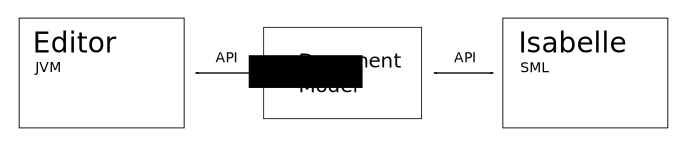
\includegraphics[width=\linewidth]{images/diagram-iscala}
  \caption{Konzept des Document Model in Isabelle/Scala}
  \captionsetup{font={footnotesize,bf,it}}
  \caption*{Vgl. \cite{iscala}}
  \label{fig:diagram-iscala}
\end{figure}

Isabelle/Scala wurde für und zusammen mit der Anwendung \textit{Isabelle/jEdit} entwickelt. JEdit
wurde hier unter anderem deswegen gewählt, weil es über sehr einfache API verfügt und somit das
Projekt nicht zu sehr auf den Editor konzentriert ist.

\TODO{Mehr Isabelle?}
